\documentclass{beamer}
\bibliographystyle{amsalpha}
\usepackage{cite}
\usepackage[normalem]{ulem}
\usepackage{fancybox}
\usepackage{enumitem}
\setitemize{label=\usebeamerfont*{itemize item}
\usebeamercolor[fg]{itemize item}
\usebeamertemplate{itemize item}}
\setbeamertemplate{footline}[frame number]{}
\setbeamertemplate{navigation symbols}{}
\graphicspath{{figures/}}



\begin{document}

	\title{Multi-Scale Plasma Modeling}
	\subtitle{Combining Molecular Dynamics with Kinetic Theory}
	\author[Price and Shohet]{Jake Price and Gil Shohet}
	\institute[CPSSW]{Computational Physics Student Summer Workshop}
	\date{August 5, 2015}
	
	\begin{frame}
		\maketitle
	\end{frame}
	
	\begin{frame}[t]{Personal Introduction}
		\vspace{2em}
		\begin{columns}
			\column[t]{0.5\linewidth}
			\centering
\includegraphics[height=0.25\textheight]{illinois.png}
			\column[t]{0.5\linewidth}
			\centering
\includegraphics[height=0.25\textheight]{stanford.png}
		\end{columns}
		\begin{columns}
			\column[t]{0.15\linewidth}
			\column[t]{0.7\linewidth}
			\begin{itemize}
				\item[] \textbf{Potential Research Interests}
				\vspace{0.5em}
				\item Multiscale modeling and simulation
				\vspace{0.5em}
				\item Model development
				\vspace{0.5em}
				\item Plasmas and nonequilibrium phenomena
			\end{itemize}
			\column[t]{0.15\linewidth}
		\end{columns}
	\end{frame}
	
	\begin{frame}{Comparison of Models}
		\begin{columns}
			\begin{column}{0.55\textwidth}
				\begin{center}\textbf{Molecular Dynamics}\end{center}\vspace{-0.8em}
				\begin{itemize}
					\item  \color{blue}Conserves total energy
					\vspace{0.5em}
					\item  Simulating particle interactions \ovalbox{``exactly''}
					\vspace{0.5em}
					\item  \color{red}Noisy, need ensemble averages
					\vspace{0.5em}
					\item  Tiny time steps
					\vspace{0.5em}
					\item  \ovalbox{Computationally expensive}
				\end{itemize}
			\end{column}
			\begin{column}{0.55\textwidth}
				\begin{center}\textbf{Kinetic Theory}\end{center}\vspace{-0.8em}
				\begin{itemize}
					\item  \color{red}Only conserves kinetic energy
					\vspace{0.5em}
					\item  Simulating particle interactions in \ovalbox{average sense}
					\vspace{0.5em}
					\item  \color{blue} Calculate bulk properties easily
					\vspace{0.5em}
					\item  Large time steps
					\vspace{0.5em}
					\item  \ovalbox{Computationally inexpensive}
				\end{itemize}
			\end{column}
		\end{columns}
		\begin{center}
			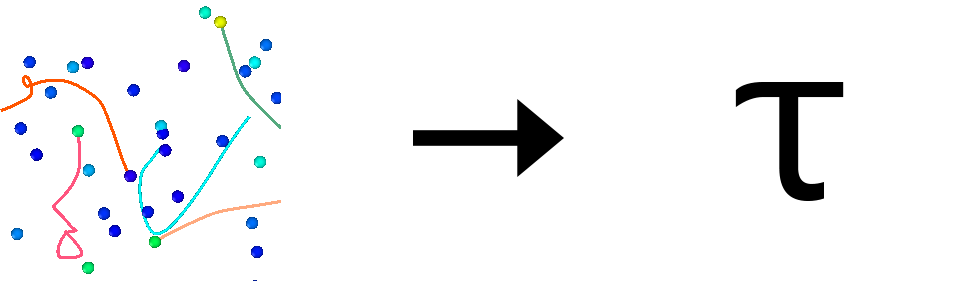
\includegraphics[height=0.3\textheight]{random_walk.png}
		\end{center}
	\end{frame}
	
	\begin{frame}{Challenges}
		\begin{itemize}
			\item[1. ]  How often do we need to update $\tau$?
			\item[2. ]  How long do we need to run the MD to recover $\tau$?
			\item[3. ]  How do we initialize the MD model from $f$?
			\item[4. ]  How do we return to the BGK model from MD?
		\end{itemize}
		\begin{center}
			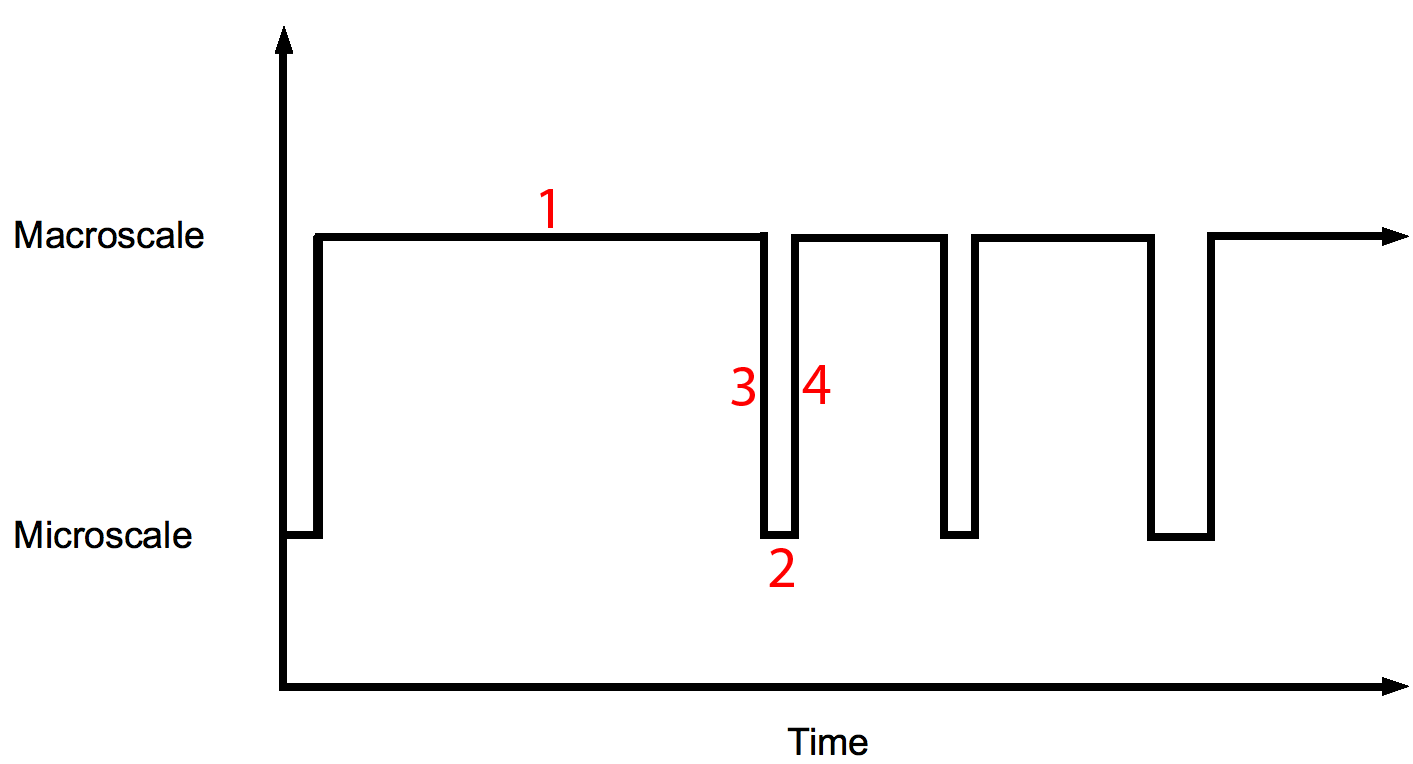
\includegraphics[height=0.55\textheight]{scheme2.png}
		\end{center}
	\end{frame}
	
	\begin{frame}{Summary}
		\begin{itemize}
			\item HMM lets us combine the accuracy of the microscale with the efficiency of the macroscale
			\vspace{1em}
			\item Connecting the models is a major challenge
			\vspace{1em}
			\begin{itemize}
				\item We have a theoretical framework and some ideas
				\vspace{1em}
				\item The ``connective tissue'' is not fully there yet
			\vspace{1em}
			\end{itemize}
			\item Tune in later to find out more!
		\end{itemize}
	\end{frame}
	
	\end{document}